\documentclass{article}

\usepackage{neurips_2026}
\usepackage[utf8]{inputenc}
\usepackage{lmodern}
\usepackage{hyperref}
\usepackage{url}
\usepackage{booktabs}
\usepackage{amsfonts}
\usepackage{amsmath}
\usepackage{amssymb}
\usepackage{nicefrac}
\usepackage{microtype}
\usepackage{xcolor}
\usepackage{graphicx}

\title{Monitorability-Aware Budgeted Process RL with Local Ambiguity Cues: A Tiny Symbolic Study}

\author{Anonymous Authors}

\begin{document}

\maketitle

\begin{abstract}
We study a tiny symbolic proxy for budgeted reasoning RL in which a controller must decide when to \texttt{THINK}, \texttt{VERIFY}, \texttt{REVISE}, or \texttt{COMMIT} under a fixed action budget. Each task is a procedurally generated arithmetic chain with exact ground truth, one optional hidden faulty step, and a noisy one-bit local ambiguity cue that is observable but not perfectly reliable. We compare random play, three heuristics, outcome-only RL, naive process-reward RL, and a monitorability-aware process reward using a tiny masked DQN trained locally on an Apple M1 laptop. On train-like depths, the proposed reward is the strongest learned method: it reaches $0.601 \pm 0.052$ success versus $0.234 \pm 0.099$ for outcome-only RL and $0.187 \pm 0.048$ for naive process RL, while also improving failed-episode localization to $0.675 \pm 0.057$ and verification recall to $0.836 \pm 0.012$. But this behavior does not robustly generalize to longer held-out chains: held-out success drops to $0.112 \pm 0.035$, below outcome-only RL at $0.132 \pm 0.055$ and far below a simple hint-triggered heuristic at $0.819 \pm 0.019$. The strongest honest claim is therefore mechanistic rather than triumphant: monitorability-aware process rewards can induce ambiguity-focused verification in-distribution, but the resulting policy is brittle under length shift.
\end{abstract}

\section{Introduction}
Recent reasoning-model work emphasizes that both train-time and test-time compute can matter for hard reasoning \citep{openai_reasoning_2024,deepseek_r1_2025}. At the same time, recent monitorability work argues that chain-of-thought traces can expose failures better than outputs alone, but that this signal may trade off against capability and may itself be fragile \citep{openai_monitorability_2025}. Anthropic's faithfulness results sharpen the caution: even when a reasoning trace is available, it need not be a faithful account of what the model actually used \citep{anthropic_faithfulness_2025}. These observations motivate a smaller question than ``does process supervision help frontier models?'': under a strict reasoning budget, when does process-aware RL help a tiny controller allocate verification effort, and when does it overfit?

We study that question in a deliberately small symbolic environment. The goal is not to chase benchmark scores or to compare against frontier language models. Instead, we construct a tiny partially observable arithmetic-chain environment with exact local checking, one optional hidden faulty transition, backtracking, a finite budget, and a noisy local ambiguity cue. The controller sees only a compact observation: normalized progress, remaining budget, a budget-slack feature, an unchecked-gap feature, the current ambiguity cue, whether it just revised, and the last verification status. This setup makes every relevant quantity exact: correctness, local fault hits, verification precision/recall, and failure localization can all be computed directly from environment state.

The core result is a structured failure mode. A simple hand-coded hint-triggered heuristic, using only the observable ambiguity cue, solves both training-depth and held-out longer chains well, so the environment does admit a strong selective-verification policy. Outcome-only RL does not reliably discover it. The proposed monitorability-aware reward does learn a more diagnostic in-distribution policy than outcome-only or naive process rewards, but this policy remains brittle under a depth shift from 3--6 training steps to 7--9 held-out steps. The resulting paper is therefore best read as a concept-and-feasibility plus negative-result study: a tiny exact proxy can isolate ambiguity-focused checking behavior, but small-budget RL still fails to recover a robust version of that behavior.

Concretely, the paper contributes three pieces: a tiny exact environment for budgeted process reasoning with local ambiguity cues, verification, and repair; a simple monitorability-aware reward that explicitly values informative verification and bounded unchecked gaps; and an empirical study showing that in-distribution ambiguity checking can improve while out-of-distribution robustness remains poor.

\section{Related Work}
\citet{openai_reasoning_2024} and \citet{deepseek_r1_2025} motivate reinforcement learning for reasoning and highlight the role of train-time and test-time compute. \citet{logic_rl_2025} argue that small, verifiable symbolic environments can reveal reasoning dynamics cheaply. We follow that spirit, but focus on a much smaller controller and a fixed budgeted control problem rather than a large language model.

For monitorability, \citet{openai_monitorability_2025} distinguish intervention, process, and outcome-property evaluations and emphasize a capability-monitorability tradeoff. Our environment is a small process-style proxy in which the trace determines whether failures remain locally diagnosable. Finally, \citet{anthropic_faithfulness_2025} show that reasoning traces need not faithfully reveal the true internal cause of a model's output. Our study does not solve faithfulness; instead, it asks whether even a perfectly instrumented symbolic proxy already exhibits a tension between solving the task and keeping failure traces locally monitorable.

\section{Problem Setup}
Each episode samples an arithmetic chain of depth $d$. Training uses $d \in \{3,\ldots,6\}$; held-out evaluation uses $d \in \{7,\ldots,9\}$. The chain is generated procedurally, so no dataset is stored. With probability $p_{\mathrm{fault}}$, exactly one transition $h \in \{1,\ldots,d\}$ is faulty. Conditional on a fault, its location is drawn from a middle-peaked prior. In addition, each step carries an observable binary ambiguity cue $c_t \in \{0,1\}$ for the current local transition. This cue is noisy: the true faulty step is flagged with high probability, but non-fault steps can also be flagged spuriously.

The controller observes only a compact partial state
\begin{equation}
o_t = \bigl(\hat{s}_t,\; \hat{b}_t,\; \hat{d},\; \hat{u}_t,\; \hat{g}_t,\; c_t,\; \rho_t,\; \ell_t\bigr),
\end{equation}
where $\hat{s}_t$ is normalized progress, $\hat{b}_t$ remaining budget, $\hat{d}$ normalized target depth, $\hat{u}_t$ normalized budget slack, $\hat{g}_t$ the normalized gap since the last checked step, $\rho_t$ indicates whether the previous action was \texttt{REVISE}, and $\ell_t \in \{\text{none}, \text{safe}, \text{unsafe}\}$ is the most recent verification outcome. The latent arithmetic state and the true fault location are never observed directly.

Available actions are \texttt{THINK}, \texttt{VERIFY}, \texttt{REVISE}, and \texttt{COMMIT}. \texttt{THINK} advances one step. \texttt{VERIFY} checks the current local transition and returns a trustworthy safe/unsafe signal. \texttt{REVISE} moves one step backward. \texttt{COMMIT} ends the episode. If the controller commits at depth $d$ with the correct latent state, the episode succeeds; otherwise it fails.

The base reward is
\begin{equation}
r_t
= \mathbb{1}\!\left[a_t=\texttt{COMMIT} \wedge \mathrm{correct}\right]
- 1.2\,\mathbb{1}\!\left[a_t=\texttt{COMMIT} \wedge \neg \mathrm{correct}\right]
- \lambda_c \, c(a_t)
+ r_t^{\mathrm{proc}},
\label{eq:reward}
\end{equation}
where $c(a_t)$ is the action cost and $\lambda_c$ is the per-action budget penalty.

We report success rate, average return, average action counts, verification precision and recall with respect to the true hidden fault, cost-adjusted accuracy, and a failed-episode localization score
\begin{equation}
\mathrm{Loc}
=
\begin{cases}
0, & \tau_{\mathrm{diag}} < h,\\
1 - \dfrac{\tau_{\mathrm{diag}} - h}{\max(1, d-h)}, & \tau_{\mathrm{diag}} \ge h,
\end{cases}
\label{eq:loc}
\end{equation}
where $h$ is the true faulty step and $\tau_{\mathrm{diag}}$ is the first step at which the trace either explicitly localizes the fault through an unsafe verification or ends at commit. High $\mathrm{Loc}$ means that failures become diagnosable near their true source rather than remaining opaque.

\section{Method}
We compare three learned reward schemes. Outcome-only RL uses $r_t^{\mathrm{proc}}=0$. Naive process RL adds a small bonus for locally valid progress and first-time useful verification, without distinguishing between high- and low-value checks. This makes it prone to weak or poorly targeted checking.

Our proposed monitorability-aware process term is
\begin{equation}
\begin{aligned}
r_t^{\mathrm{proc}}
=\;& \lambda_{\mathrm{safe}} \,\mathbb{1}[v_t^{\mathrm{safe}}]
+ \lambda_{\mathrm{fault}} \,\mathbb{1}[v_t^{\mathrm{fault}}] \\
& + \lambda_{\mathrm{hint}} \,\mathbb{1}[a_t=\texttt{VERIFY} \wedge c_t = 1 \wedge \neg w_t] \\
& - \lambda_{\mathrm{waste}} \,\mathbb{1}[w_t]
- \lambda_{\mathrm{gap}} \frac{g_t - g_{t-1}}{\max(1,d)},
\end{aligned}
\label{eq:monitorability}
\end{equation}
Here $v_t^{\mathrm{safe}}$ denotes a first-time safe verification on a locally valid step, $v_t^{\mathrm{fault}}$ a first-time unsafe verification that hits the true faulty transition, $w_t$ a repeated or otherwise uninformative verification, and $g_t$ the unchecked gap between the current step and the most recently checked step. The ambiguity-aware term rewards spending verification budget on locally flagged ambiguous steps rather than on uniformly low-signal checks.

RL uses a tiny masked Double DQN with a two-layer MLP and discrete action masking. Let $Q_{\theta}(o,a)$ be the online network and $Q_{\bar{\theta}}$ the target network. We minimize the standard one-step temporal-difference loss
\begin{equation}
\mathcal{L}(\theta)
= \mathbb{E}\Bigl[\bigl(Q_{\theta}(o_t,a_t) - y_t\bigr)^2\Bigr],
\qquad
y_t = r_t + \gamma (1-d_t)\, Q_{\bar{\theta}}\!\left(o_{t+1}, \arg\max_{a'} Q_{\theta}(o_{t+1},a')\right),
\label{eq:dqn}
\end{equation}
with $\gamma=0.99$. The network is intentionally tiny; the point of the study is reward design and failure analysis under a small compute budget, not scaling.

\section{Experimental Setup}
The default environment uses training depths 3--6, held-out depths 7--9, fault probability $p_{\mathrm{fault}}=0.8$, unit action costs, and a budget equal to depth plus six extra actions. The ambiguity cue flags the true faulty step with high probability and produces occasional false positives on non-fault steps. We evaluate random play, \texttt{Always THINK}, \texttt{Verify Every Step}, a hand-coded \texttt{Hint-Triggered Heuristic}, outcome-only RL, naive process RL, and monitorability-aware RL. We also train four ablations of the proposed method: no budget penalty, no \texttt{VERIFY}, no \texttt{REVISE}, and no monitorability term.

The full experiment uses five random seeds unless otherwise stated, with 300 procedurally generated evaluation episodes per seed and setting. All runs are local and CPU-compatible; the reported experiments were executed on a MacBook Air with an Apple M1 chip. The repository remains well under the 1\,GB footprint target and requires no external datasets, pretrained models, or cloud resources.

\section{Results}
\subsection{A strong selective policy exists}
The first important sanity check is that the environment does support a strong policy. The hint-triggered heuristic, which uses only the observable ambiguity cue and no privileged access to hidden state, reaches $0.827 \pm 0.012$ success on train-like depths and $0.819 \pm 0.019$ on held-out longer chains. This matters because it rules out a trivial explanation for RL failure: the task itself is not impossible under the imposed budget. Selective ambiguity-focused verification is available; the learned policies simply do not recover it robustly.

\subsection{Monitorability-aware RL helps in-distribution}
On train-like depths, the monitorability-aware reward is the strongest learned method. It reaches $0.601 \pm 0.052$ success, compared with $0.234 \pm 0.099$ for outcome-only RL and $0.187 \pm 0.048$ for naive process RL. It also checks much more effectively than outcome-only RL, with verification recall $0.836 \pm 0.012$ versus $0.318 \pm 0.131$, and it raises failed-episode localization from $0.259 \pm 0.116$ to $0.675 \pm 0.057$. Relative to the naive process reward, it not only succeeds more often but also localizes failures more cleanly ($0.675$ versus $0.152$). This is the main positive result of the paper: explicit ambiguity-aware process rewards can induce short-horizon checking behavior in a tiny controller.

Figure~\ref{fig:main} and Table~\ref{tab:main} summarize the main comparison. Two patterns matter more than raw score. First, monitorability-aware RL is much more diagnostic than outcome-only RL: it checks more often, localizes failures earlier, and attains much higher verification recall. Second, a large gap remains between the learned policy and the simple hint-triggered heuristic, which means the learned controller is still only partially exploiting the available cue.

The ablations sharpen this point. On train-like depths, the full proposed reward is stronger than its monitorability ablations: removing the budget penalty lowers success to $0.479 \pm 0.077$, removing the monitorability term lowers it to $0.520 \pm 0.081$, removing \texttt{REVISE} lowers it to $0.186 \pm 0.009$, and removing \texttt{VERIFY} collapses to zero. In-distribution, the complete reward is therefore not just different but genuinely useful.

\begin{table}[t]
\centering
\small
\setlength{\tabcolsep}{3pt}
\caption{Main metrics on train-like and held-out longer depths.}
\label{tab:main}
\resizebox{\linewidth}{!}{\begin{tabular}{lccccc}
\toprule
Method & Success 3--6 & Success 7--9 & Success 10--14 & Detect 7--9 & Cost-adj. 7--9 \\
\midrule
Random & 0.00\,{\scriptsize[0.00, 0.01]} & 0.00\,{\scriptsize[0.00, 0.00]} & 0.00\,{\scriptsize[0.00, 0.00]} & 0.02\,{\scriptsize[0.01, 0.02]} & -0.09\,{\scriptsize[-0.09, -0.08]} \\
Always THINK & 0.20\,{\scriptsize[0.19, 0.21]} & 0.20\,{\scriptsize[0.19, 0.21]} & 0.20\,{\scriptsize[0.19, 0.21]} & 0.00\,{\scriptsize[0.00, 0.00]} & -0.20\,{\scriptsize[-0.21, -0.19]} \\
Verify every step & 0.80\,{\scriptsize[0.79, 0.81]} & 0.06\,{\scriptsize[0.06, 0.07]} & 0.00\,{\scriptsize[0.00, 0.00]} & 0.93\,{\scriptsize[0.92, 0.94]} & -0.63\,{\scriptsize[-0.64, -0.63]} \\
Cue-triggered & 0.87\,{\scriptsize[0.87, 0.88]} & 0.88\,{\scriptsize[0.87, 0.89]} & 0.85\,{\scriptsize[0.84, 0.86]} & 0.85\,{\scriptsize[0.84, 0.87]} & 0.33\,{\scriptsize[0.31, 0.34]} \\
Budget-aware & 0.97\,{\scriptsize[0.96, 0.97]} & 0.82\,{\scriptsize[0.81, 0.84]} & 0.68\,{\scriptsize[0.66, 0.70]} & 0.78\,{\scriptsize[0.76, 0.79]} & 0.19\,{\scriptsize[0.17, 0.20]} \\
\midrule
Outcome (inv) & 0.72\,{\scriptsize[0.65, 0.79]} & 0.62\,{\scriptsize[0.50, 0.73]} & 0.52\,{\scriptsize[0.40, 0.65]} & 0.61\,{\scriptsize[0.45, 0.75]} & -0.02\,{\scriptsize[-0.14, 0.09]} \\
Naive process (inv) & 0.85\,{\scriptsize[0.81, 0.89]} & 0.76\,{\scriptsize[0.65, 0.84]} & 0.65\,{\scriptsize[0.54, 0.75]} & 0.76\,{\scriptsize[0.63, 0.86]} & 0.09\,{\scriptsize[-0.01, 0.18]} \\
Monitorability (inv) & 0.91\,{\scriptsize[0.89, 0.92]} & 0.86\,{\scriptsize[0.84, 0.89]} & 0.74\,{\scriptsize[0.69, 0.79]} & 0.85\,{\scriptsize[0.83, 0.87]} & 0.19\,{\scriptsize[0.15, 0.22]} \\
Outcome (abs) & 0.34\,{\scriptsize[0.29, 0.39]} & 0.16\,{\scriptsize[0.09, 0.22]} & 0.05\,{\scriptsize[0.00, 0.11]} & 0.09\,{\scriptsize[0.04, 0.16]} & -0.27\,{\scriptsize[-0.36, -0.17]} \\
Naive process (abs) & 0.44\,{\scriptsize[0.33, 0.52]} & 0.16\,{\scriptsize[0.10, 0.22]} & 0.03\,{\scriptsize[0.00, 0.06]} & 0.30\,{\scriptsize[0.14, 0.49]} & -0.32\,{\scriptsize[-0.42, -0.23]} \\
Monitorability (abs) & 0.76\,{\scriptsize[0.73, 0.79]} & 0.31\,{\scriptsize[0.22, 0.39]} & 0.03\,{\scriptsize[0.00, 0.07]} & 0.60\,{\scriptsize[0.46, 0.72]} & -0.24\,{\scriptsize[-0.32, -0.18]} \\
\bottomrule
\end{tabular}
}
\end{table}

\begin{figure}[t]
\centering
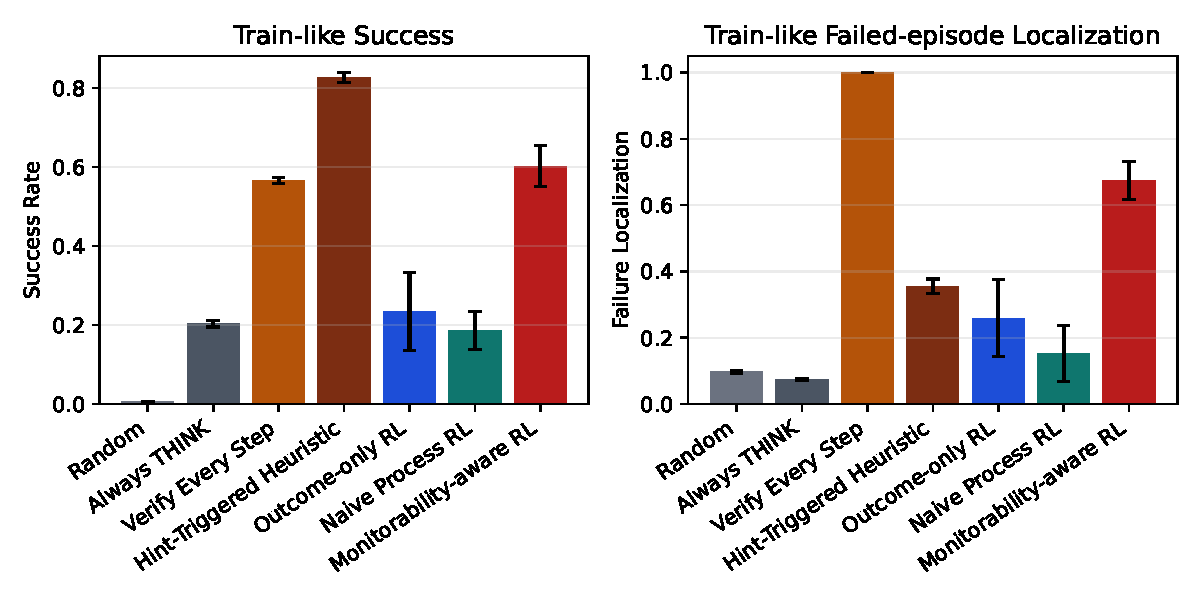
\includegraphics[width=\linewidth]{figures/method_comparison.pdf}
\caption{Main train-like comparison. A strong hand-coded hint-triggered policy exists; monitorability-aware RL improves checking behavior relative to learned baselines but does not close the gap.}
\label{fig:main}
\end{figure}

\subsection{The gain is brittle under length shift}
The main negative result appears under the depth shift from 3--6 training steps to 7--9 held-out steps. The monitorability-aware policy keeps much better diagnostic behavior than outcome-only RL, with failure localization $0.556 \pm 0.083$ versus $0.119 \pm 0.054$ and verification recall $0.555 \pm 0.080$ versus $0.123 \pm 0.060$. But it does not preserve its train-like success: held-out success falls to $0.112 \pm 0.035$, slightly below outcome-only RL at $0.132 \pm 0.055$ and far below the hint-triggered heuristic at $0.819 \pm 0.019$. Instead, the learned policy spends budget on ambiguity-focused checking without recovering a robust long-horizon repair policy.

This creates a clean mechanism story rather than a clean algorithmic win. Process-aware shaping can indeed move the learned policy toward ambiguity-focused verification. But the learned controller overfits the short-horizon budget regime: it learns to check, yet fails to translate that checking into a reliable longer-chain repair-and-commit strategy.

The held-out ablations support that interpretation. Removing the budget penalty raises held-out success from $0.112 \pm 0.035$ to $0.291 \pm 0.090$, though cost-adjusted accuracy remains negative. Removing the explicit monitorability term also improves held-out success to $0.225 \pm 0.031$. By contrast, removing \texttt{VERIFY} collapses held-out success to zero, while removing \texttt{REVISE} yields only $0.139 \pm 0.019$. The full proposed shaping is therefore best viewed as an in-distribution inducer of checking behavior that over-commits to that behavior under length shift.

\begin{figure}[t]
\centering
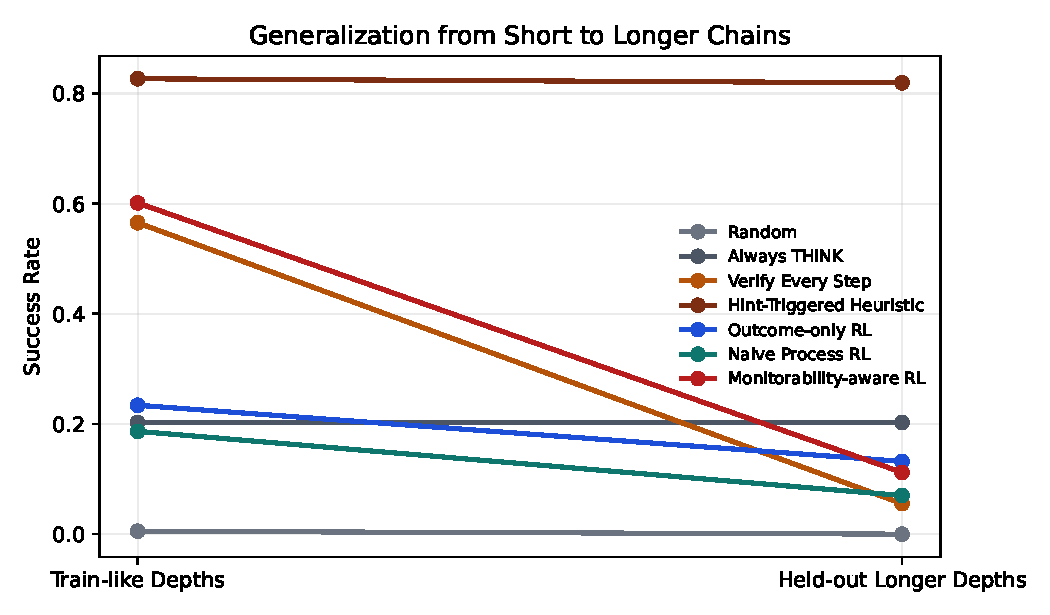
\includegraphics[width=\linewidth]{figures/generalization.pdf}
\caption{Generalization from short training chains to longer held-out chains. The monitorability-aware policy learns a stronger in-distribution checking strategy, but this behavior does not transfer robustly to longer reasoning chains.}
\label{fig:gen}
\end{figure}

\subsection{Cost and budget sensitivity remain sharp}
The held-out tradeoff plot in Figure~\ref{fig:tradeoff} shows that verification remains budget-sensitive even after adding the ambiguity cue. Increasing verification cost quickly degrades the learned ambiguity-checking policy. Likewise, more budget helps the hint-triggered heuristic substantially, but the learned monitorability-aware policy does not fully capitalize on that slack. This is consistent with the broader interpretation of the paper: the environment makes the intended policy available, yet small-scale RL still struggles to learn a version that is both selective and robust.

\begin{figure}[t]
\centering
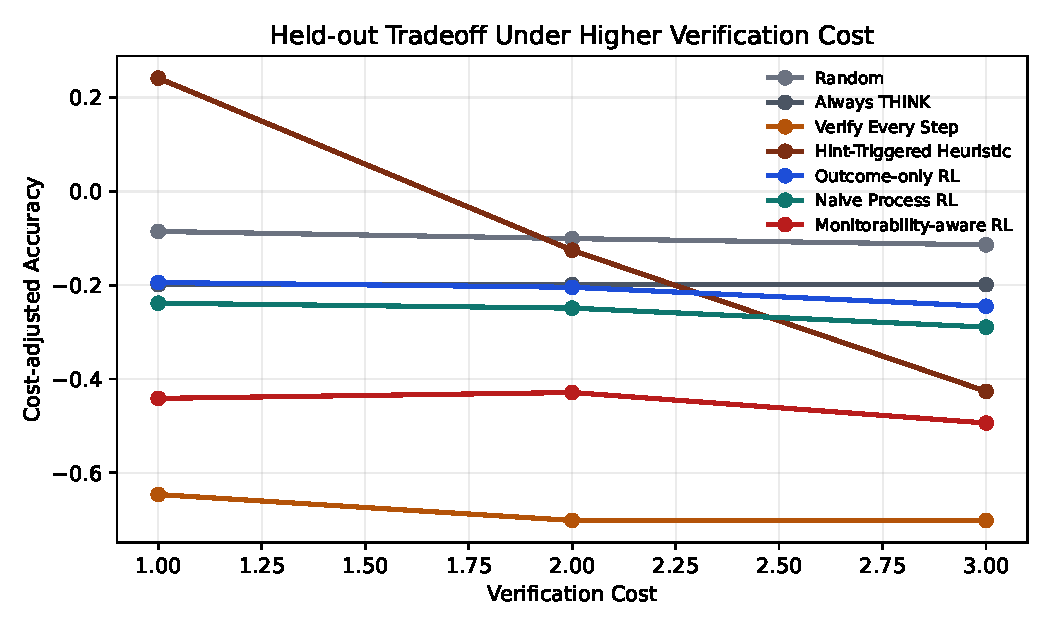
\includegraphics[width=\linewidth]{figures/tradeoff_verify_cost.pdf}
\caption{Held-out cost-adjusted accuracy versus verification cost. The learned process-aware policy is still brittle: stronger ambiguity checking does not automatically translate into robust longer-horizon control.}
\label{fig:tradeoff}
\end{figure}

\section{Discussion}
The point of this environment is not its raw difficulty. The useful property is that it isolates a concrete decision: when the current local step looks ambiguous, should the controller spend scarce budget to verify now, move forward, or backtrack? Because the environment has exact ground truth, we can distinguish three things cleanly: whether the controller solved the task, whether it checked the right local steps, and whether failures stayed locally diagnosable.

In that sense the paper succeeds as a mechanism study. The ambiguity cue is enough to support a strong selective-verification heuristic. A monitorability-aware reward can push a learned policy toward that kind of checking. But the learned controller still fails to recover the heuristic robustly, especially on longer chains. This makes the project a better fit for Concept \& Feasibility or Negative Results than for a strong main-track method claim.

\section{Limitations}
This work remains intentionally tiny. The controller is a small MLP over a symbolic state, not a language model; the environment contains at most one hidden fault; the ambiguity cue is hand-designed; and the local arithmetic-chain abstraction does not capture the semantic ambiguity or strategic concealment that matter in real chain-of-thought settings. The hint-triggered heuristic also shows that part of the difficulty here is simply learning a short program from small-budget RL, not discovering a fundamentally unavailable strategy.

The empirical limitation is more important: the learned monitorability-aware policy does look promising in-distribution, but it still fails under a simple length shift. The strongest honest conclusion is not that the proposed reward solves budgeted process supervision, but that it reveals a sharp overfitting mode in tiny process-aware RL.

\section{Conclusion}
We introduced a tiny symbolic environment for studying budgeted process supervision with exact local checking, backtracking, and noisy ambiguity cues. In this proxy, ambiguity-aware process rewards can induce in-distribution checking behavior, but the resulting policies remain brittle under longer held-out chains. The main contribution is therefore diagnostic: exact small-scale environments can reveal how process rewards shape verification behavior, and can show clearly when those gains fail to become robust reasoning improvements.

\bibliographystyle{plainnat}
\bibliography{references}

\appendix

\section{Additional Experimental Details}
Training uses a tiny masked Double DQN with 64 hidden units per layer and Adam with learning rate $10^{-3}$. The full run uses five random seeds, 5000 training episodes per seed and variant, and 300 evaluation episodes per seed and setting. All tasks are procedurally generated online.

\section{Additional Diagnostics}
Figure~\ref{fig:diag} reports train-like verification precision and recall. The proposed reward should be read jointly with the main success and localization metrics: high recall alone is not enough, because verify-every-step remains inefficient, while a low-checking outcome-only policy can miss most faults entirely.

\begin{figure}[h]
\centering
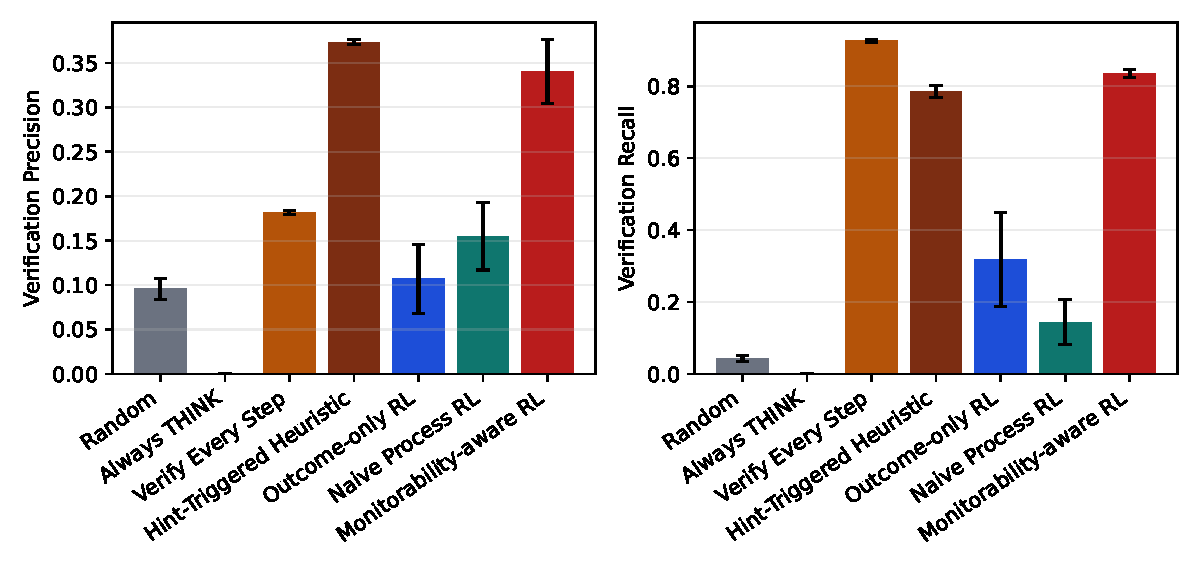
\includegraphics[width=\linewidth]{figures/verification_diagnostics.pdf}
\caption{Verification precision and recall on train-like tasks. Process-aware rewards improve checking behavior, but not all checking policies convert diagnostics into successful longer-horizon control.}
\label{fig:diag}
\end{figure}

\section{External Assets}
The paper uses the official NeurIPS 2026 style bundle from \url{https://neurips.cc}, the \texttt{lineno} package under the \LaTeX{} Project Public License, and the Latin Modern font package under the GUST Font License / LPPL terms. The experiments use only the Python dependencies listed in \texttt{requirements.txt}; no external datasets, pretrained models, or proprietary APIs are required.

\section*{NeurIPS Paper Checklist}

\begin{enumerate}

\item {\bf Claims}
    \item[] Question: Do the main claims made in the abstract and introduction accurately reflect the paper's contributions and scope?
    \item[] Answer: \answerYes{}
    \item[] Justification: The abstract and introduction explicitly present the work as a tiny symbolic proxy and state the main result as an in-distribution monitorability gain that does not generalize to longer chains.
    \item[] Guidelines:
    \begin{itemize}
        \item The answer \answerNA{} means that the abstract and introduction do not include the claims made in the paper.
        \item The abstract and/or introduction should clearly state the claims made, including the contributions made in the paper and important assumptions and limitations. A \answerNo{} or \answerNA{} answer to this question will not be perceived well by the reviewers. 
        \item The claims made should match theoretical and experimental results, and reflect how much the results can be expected to generalize to other settings. 
        \item It is fine to include aspirational goals as motivation as long as it is clear that these goals are not attained by the paper. 
    \end{itemize}

\item {\bf Limitations}
    \item[] Question: Does the paper discuss the limitations of the work performed by the authors?
    \item[] Answer: \answerYes{}
    \item[] Justification: Section ``Limitations'' explicitly discusses the narrow symbolic environment, hand-designed ambiguity cue, tiny masked Double DQN controller, and the weak out-of-distribution results.
    \item[] Guidelines:
    \begin{itemize}
        \item The answer \answerNA{} means that the paper has no limitation while the answer \answerNo{} means that the paper has limitations, but those are not discussed in the paper. 
        \item The authors are encouraged to create a separate ``Limitations'' section in their paper.
        \item The paper should point out any strong assumptions and how robust the results are to violations of these assumptions (e.g., independence assumptions, noiseless settings, model well-specification, asymptotic approximations only holding locally). The authors should reflect on how these assumptions might be violated in practice and what the implications would be.
        \item The authors should reflect on the scope of the claims made, e.g., if the approach was only tested on a few datasets or with a few runs. In general, empirical results often depend on implicit assumptions, which should be articulated.
        \item The authors should reflect on the factors that influence the performance of the approach. For example, a facial recognition algorithm may perform poorly when image resolution is low or images are taken in low lighting. Or a speech-to-text system might not be used reliably to provide closed captions for online lectures because it fails to handle technical jargon.
        \item The authors should discuss the computational efficiency of the proposed algorithms and how they scale with dataset size.
        \item If applicable, the authors should discuss possible limitations of their approach to address problems of privacy and fairness.
        \item While the authors might fear that complete honesty about limitations might be used by reviewers as grounds for rejection, a worse outcome might be that reviewers discover limitations that aren't acknowledged in the paper. The authors should use their best judgment and recognize that individual actions in favor of transparency play an important role in developing norms that preserve the integrity of the community. Reviewers will be specifically instructed to not penalize honesty concerning limitations.
    \end{itemize}

\item {\bf Theory assumptions and proofs}
    \item[] Question: For each theoretical result, does the paper provide the full set of assumptions and a complete (and correct) proof?
    \item[] Answer: \answerNA{}
    \item[] Justification: The paper is empirical and does not claim a formal theorem or proof.
    \item[] Guidelines:
    \begin{itemize}
        \item The answer \answerNA{} means that the paper does not include theoretical results. 
        \item All the theorems, formulas, and proofs in the paper should be numbered and cross-referenced.
        \item All assumptions should be clearly stated or referenced in the statement of any theorems.
        \item The proofs can either appear in the main paper or the supplemental material, but if they appear in the supplemental material, the authors are encouraged to provide a short proof sketch to provide intuition. 
        \item Inversely, any informal proof provided in the core of the paper should be complemented by formal proofs provided in appendix or supplemental material.
        \item Theorems and Lemmas that the proof relies upon should be properly referenced. 
    \end{itemize}

    \item {\bf Experimental result reproducibility}
    \item[] Question: Does the paper fully disclose all the information needed to reproduce the main experimental results of the paper to the extent that it affects the main claims and/or conclusions of the paper (regardless of whether the code and data are provided or not)?
    \item[] Answer: \answerYes{}
    \item[] Justification: Sections ``Problem Setup,'' ``Method,'' ``Experimental Setup,'' and the appendix specify the environment, reward functions, learner, seeds, and evaluation protocol, and the repository includes runnable scripts and raw CSV outputs.
    \item[] Guidelines:
    \begin{itemize}
        \item The answer \answerNA{} means that the paper does not include experiments.
        \item If the paper includes experiments, a \answerNo{} answer to this question will not be perceived well by the reviewers: Making the paper reproducible is important, regardless of whether the code and data are provided or not.
        \item If the contribution is a dataset and\slash or model, the authors should describe the steps taken to make their results reproducible or verifiable. 
        \item Depending on the contribution, reproducibility can be accomplished in various ways. For example, if the contribution is a novel architecture, describing the architecture fully might suffice, or if the contribution is a specific model and empirical evaluation, it may be necessary to either make it possible for others to replicate the model with the same dataset, or provide access to the model. In general. releasing code and data is often one good way to accomplish this, but reproducibility can also be provided via detailed instructions for how to replicate the results, access to a hosted model (e.g., in the case of a large language model), releasing of a model checkpoint, or other means that are appropriate to the research performed.
        \item While NeurIPS does not require releasing code, the conference does require all submissions to provide some reasonable avenue for reproducibility, which may depend on the nature of the contribution. For example
        \begin{enumerate}
            \item If the contribution is primarily a new algorithm, the paper should make it clear how to reproduce that algorithm.
            \item If the contribution is primarily a new model architecture, the paper should describe the architecture clearly and fully.
            \item If the contribution is a new model (e.g., a large language model), then there should either be a way to access this model for reproducing the results or a way to reproduce the model (e.g., with an open-source dataset or instructions for how to construct the dataset).
            \item We recognize that reproducibility may be tricky in some cases, in which case authors are welcome to describe the particular way they provide for reproducibility. In the case of closed-source models, it may be that access to the model is limited in some way (e.g., to registered users), but it should be possible for other researchers to have some path to reproducing or verifying the results.
        \end{enumerate}
    \end{itemize}


\item {\bf Open access to data and code}
    \item[] Question: Does the paper provide open access to the data and code, with sufficient instructions to faithfully reproduce the main experimental results, as described in supplemental material?
    \item[] Answer: \answerYes{}
    \item[] Justification: The project uses no external dataset, and the repository includes the full source, configs, scripts, figures, tables, and reproduction commands described in the appendix and README.
    \item[] Guidelines:
    \begin{itemize}
        \item The answer \answerNA{} means that paper does not include experiments requiring code.
        \item Please see the NeurIPS code and data submission guidelines (\url{https://neurips.cc/public/guides/CodeSubmissionPolicy}) for more details.
        \item While we encourage the release of code and data, we understand that this might not be possible, so \answerNo{} is an acceptable answer. Papers cannot be rejected simply for not including code, unless this is central to the contribution (e.g., for a new open-source benchmark).
        \item The instructions should contain the exact command and environment needed to run to reproduce the results. See the NeurIPS code and data submission guidelines (\url{https://neurips.cc/public/guides/CodeSubmissionPolicy}) for more details.
        \item The authors should provide instructions on data access and preparation, including how to access the raw data, preprocessed data, intermediate data, and generated data, etc.
        \item The authors should provide scripts to reproduce all experimental results for the new proposed method and baselines. If only a subset of experiments are reproducible, they should state which ones are omitted from the script and why.
        \item At submission time, to preserve anonymity, the authors should release anonymized versions (if applicable).
        \item Providing as much information as possible in supplemental material (appended to the paper) is recommended, but including URLs to data and code is permitted.
    \end{itemize}


\item {\bf Experimental setting/details}
    \item[] Question: Does the paper specify all the training and test details (e.g., data splits, hyperparameters, how they were chosen, type of optimizer) necessary to understand the results?
    \item[] Answer: \answerYes{}
    \item[] Justification: Section ``Experimental Setup'' gives the train/test depth split, budgets, reward settings, seed count, and hardware, while the appendix records the masked Double DQN and reward hyperparameters.
    \item[] Guidelines:
    \begin{itemize}
        \item The answer \answerNA{} means that the paper does not include experiments.
        \item The experimental setting should be presented in the core of the paper to a level of detail that is necessary to appreciate the results and make sense of them.
        \item The full details can be provided either with the code, in appendix, or as supplemental material.
    \end{itemize}

\item {\bf Experiment statistical significance}
    \item[] Question: Does the paper report error bars suitably and correctly defined or other appropriate information about the statistical significance of the experiments?
    \item[] Answer: \answerYes{}
    \item[] Justification: Tables and figures report mean \(\pm\) standard error over five random seeds, and the experimental setup section states the seed count and evaluation protocol.
    \item[] Guidelines:
    \begin{itemize}
        \item The answer \answerNA{} means that the paper does not include experiments.
        \item The authors should answer \answerYes{} if the results are accompanied by error bars, confidence intervals, or statistical significance tests, at least for the experiments that support the main claims of the paper.
        \item The factors of variability that the error bars are capturing should be clearly stated (for example, train/test split, initialization, random drawing of some parameter, or overall run with given experimental conditions).
        \item The method for calculating the error bars should be explained (closed form formula, call to a library function, bootstrap, etc.)
        \item The assumptions made should be given (e.g., Normally distributed errors).
        \item It should be clear whether the error bar is the standard deviation or the standard error of the mean.
        \item It is OK to report 1-sigma error bars, but one should state it. The authors should preferably report a 2-sigma error bar than state that they have a 96\% CI, if the hypothesis of Normality of errors is not verified.
        \item For asymmetric distributions, the authors should be careful not to show in tables or figures symmetric error bars that would yield results that are out of range (e.g., negative error rates).
        \item If error bars are reported in tables or plots, the authors should explain in the text how they were calculated and reference the corresponding figures or tables in the text.
    \end{itemize}

\item {\bf Experiments compute resources}
    \item[] Question: For each experiment, does the paper provide sufficient information on the computer resources (type of compute workers, memory, time of execution) needed to reproduce the experiments?
    \item[] Answer: \answerYes{}
    \item[] Justification: Section ``Experimental Setup'' and Appendix Table~\ref{tab:hparams} report the Apple M1 laptop, CPU compatibility, model size, training and evaluation episode counts, and repository footprint.
    \item[] Guidelines:
    \begin{itemize}
        \item The answer \answerNA{} means that the paper does not include experiments.
        \item The paper should indicate the type of compute workers CPU or GPU, internal cluster, or cloud provider, including relevant memory and storage.
        \item The paper should provide the amount of compute required for each of the individual experimental runs as well as estimate the total compute. 
        \item The paper should disclose whether the full research project required more compute than the experiments reported in the paper (e.g., preliminary or failed experiments that didn't make it into the paper). 
    \end{itemize}
    
\item {\bf Code of ethics}
    \item[] Question: Does the research conducted in the paper conform, in every respect, with the NeurIPS Code of Ethics \url{https://neurips.cc/public/EthicsGuidelines}?
    \item[] Answer: \answerYes{}
    \item[] Justification: The project uses only synthetic arithmetic tasks, does not involve human subjects, personal data, external APIs, or unsafe model release, and is presented with explicit limitations.
    \item[] Guidelines:
    \begin{itemize}
        \item The answer \answerNA{} means that the authors have not reviewed the NeurIPS Code of Ethics.
        \item If the authors answer \answerNo, they should explain the special circumstances that require a deviation from the Code of Ethics.
        \item The authors should make sure to preserve anonymity (e.g., if there is a special consideration due to laws or regulations in their jurisdiction).
    \end{itemize}


\item {\bf Broader impacts}
    \item[] Question: Does the paper discuss both potential positive societal impacts and negative societal impacts of the work performed?
    \item[] Answer: \answerYes{}
    \item[] Justification: Section ``Limitations'' notes both the value of cheap exact testbeds and the negative risk of over-interpreting toy monitorability results as evidence about real model faithfulness.
    \item[] Guidelines:
    \begin{itemize}
        \item The answer \answerNA{} means that there is no societal impact of the work performed.
        \item If the authors answer \answerNA{} or \answerNo, they should explain why their work has no societal impact or why the paper does not address societal impact.
        \item Examples of negative societal impacts include potential malicious or unintended uses (e.g., disinformation, generating fake profiles, surveillance), fairness considerations (e.g., deployment of technologies that could make decisions that unfairly impact specific groups), privacy considerations, and security considerations.
        \item The conference expects that many papers will be foundational research and not tied to particular applications, let alone deployments. However, if there is a direct path to any negative applications, the authors should point it out. For example, it is legitimate to point out that an improvement in the quality of generative models could be used to generate Deepfakes for disinformation. On the other hand, it is not needed to point out that a generic algorithm for optimizing neural networks could enable people to train models that generate Deepfakes faster.
        \item The authors should consider possible harms that could arise when the technology is being used as intended and functioning correctly, harms that could arise when the technology is being used as intended but gives incorrect results, and harms following from (intentional or unintentional) misuse of the technology.
        \item If there are negative societal impacts, the authors could also discuss possible mitigation strategies (e.g., gated release of models, providing defenses in addition to attacks, mechanisms for monitoring misuse, mechanisms to monitor how a system learns from feedback over time, improving the efficiency and accessibility of ML).
    \end{itemize}
    
\item {\bf Safeguards}
    \item[] Question: Does the paper describe safeguards that have been put in place for responsible release of data or models that have a high risk for misuse (e.g., pre-trained language models, image generators, or scraped datasets)?
    \item[] Answer: \answerNA{}
    \item[] Justification: The release contains only small symbolic environment code, figures, and paper assets; it does not release a pretrained model, scraped dataset, or high-risk artifact.
    \item[] Guidelines:
    \begin{itemize}
        \item The answer \answerNA{} means that the paper poses no such risks.
        \item Released models that have a high risk for misuse or dual-use should be released with necessary safeguards to allow for controlled use of the model, for example by requiring that users adhere to usage guidelines or restrictions to access the model or implementing safety filters. 
        \item Datasets that have been scraped from the Internet could pose safety risks. The authors should describe how they avoided releasing unsafe images.
        \item We recognize that providing effective safeguards is challenging, and many papers do not require this, but we encourage authors to take this into account and make a best faith effort.
    \end{itemize}

\item {\bf Licenses for existing assets}
    \item[] Question: Are the creators or original owners of assets (e.g., code, data, models), used in the paper, properly credited and are the license and terms of use explicitly mentioned and properly respected?
    \item[] Answer: \answerYes{}
    \item[] Justification: The appendix names the external assets used directly in the submission package, including the official NeurIPS style bundle, the \texttt{lineno} package under LPPL, and Latin Modern under the GUST Font License / LPPL terms.
    \item[] Guidelines:
    \begin{itemize}
        \item The answer \answerNA{} means that the paper does not use existing assets.
        \item The authors should cite the original paper that produced the code package or dataset.
        \item The authors should state which version of the asset is used and, if possible, include a URL.
        \item The name of the license (e.g., CC-BY 4.0) should be included for each asset.
        \item For scraped data from a particular source (e.g., website), the copyright and terms of service of that source should be provided.
        \item If assets are released, the license, copyright information, and terms of use in the package should be provided. For popular datasets, \url{paperswithcode.com/datasets} has curated licenses for some datasets. Their licensing guide can help determine the license of a dataset.
        \item For existing datasets that are re-packaged, both the original license and the license of the derived asset (if it has changed) should be provided.
        \item If this information is not available online, the authors are encouraged to reach out to the asset's creators.
    \end{itemize}

\item {\bf New assets}
    \item[] Question: Are new assets introduced in the paper well documented and is the documentation provided alongside the assets?
    \item[] Answer: \answerYes{}
    \item[] Justification: The new assets are the environment, training/evaluation scripts, result CSVs, figures, and paper source; they are documented in the paper, appendix, and repository README.
    \item[] Guidelines:
    \begin{itemize}
        \item The answer \answerNA{} means that the paper does not release new assets.
        \item Researchers should communicate the details of the dataset\slash code\slash model as part of their submissions via structured templates. This includes details about training, license, limitations, etc. 
        \item The paper should discuss whether and how consent was obtained from people whose asset is used.
        \item At submission time, remember to anonymize your assets (if applicable). You can either create an anonymized URL or include an anonymized zip file.
    \end{itemize}

\item {\bf Crowdsourcing and research with human subjects}
    \item[] Question: For crowdsourcing experiments and research with human subjects, does the paper include the full text of instructions given to participants and screenshots, if applicable, as well as details about compensation (if any)? 
    \item[] Answer: \answerNA{}
    \item[] Justification: The work does not involve crowdsourcing or human subjects.
    \item[] Guidelines:
    \begin{itemize}
        \item The answer \answerNA{} means that the paper does not involve crowdsourcing nor research with human subjects.
        \item Including this information in the supplemental material is fine, but if the main contribution of the paper involves human subjects, then as much detail as possible should be included in the main paper. 
        \item According to the NeurIPS Code of Ethics, workers involved in data collection, curation, or other labor should be paid at least the minimum wage in the country of the data collector. 
    \end{itemize}

\item {\bf Institutional review board (IRB) approvals or equivalent for research with human subjects}
    \item[] Question: Does the paper describe potential risks incurred by study participants, whether such risks were disclosed to the subjects, and whether Institutional Review Board (IRB) approvals (or an equivalent approval/review based on the requirements of your country or institution) were obtained?
    \item[] Answer: \answerNA{}
    \item[] Justification: The project contains no human-subject data collection or experimentation.
    \item[] Guidelines:
    \begin{itemize}
        \item The answer \answerNA{} means that the paper does not involve crowdsourcing nor research with human subjects.
        \item Depending on the country in which research is conducted, IRB approval (or equivalent) may be required for any human subjects research. If you obtained IRB approval, you should clearly state this in the paper. 
        \item We recognize that the procedures for this may vary significantly between institutions and locations, and we expect authors to adhere to the NeurIPS Code of Ethics and the guidelines for their institution. 
        \item For initial submissions, do not include any information that would break anonymity (if applicable), such as the institution conducting the review.
    \end{itemize}

\item {\bf Declaration of LLM usage}
    \item[] Question: Does the paper describe the usage of LLMs if it is an important, original, or non-standard component of the core methods in this research? Note that if the LLM is used only for writing, editing, or formatting purposes and does \emph{not} impact the core methodology, scientific rigor, or originality of the research, declaration is not required.
    %this research? 
    \item[] Answer: \answerNA{}
    \item[] Justification: No large language model is part of the reported environment, learner, reward design, or evaluation pipeline; the core method is a symbolic environment with a tiny masked Double DQN.
    \item[] Guidelines:
    \begin{itemize}
        \item The answer \answerNA{} means that the core method development in this research does not involve LLMs as any important, original, or non-standard components.
        \item Please refer to our LLM policy in the NeurIPS handbook for what should or should not be described.
    \end{itemize}

\end{enumerate}


\end{document}
